%!TEX root=../oi-magistr-si.tex
\section[TVS - Formální specifikace programu, model checking]{Formální specifikace programu. Verifikace pomocí metod automatického dokazování a metody model-checking.}

Cíle kladené na požadavky specifikace. Musí být demonstrováno že požadavky jsou \hl{správné, úplné, přesné, konzistentní a testovatelné}. Díky takto nadefinovaným požadavkům můžeme SW vefirikovat

\paragraph{Formální verifikace} je technika založená na formálních metodách. Využívá matematicky založené jazyky, které umožňují \textbf{specifikaci} a \textbf{verifikaci} systémů:
\begin{itemize}[itemsep=0px]
\item specifikace = zapsání požadavků na systém v matematickém jazyce
\item verifikace = formální důkaz toho, že splňuje požadavky
\end{itemize}

Na vstupu dostáváme (matematický) model systému ($M$) a specifikaci požadavků kladených na systém v podobě formulí $\phi$ určité temporální logiky.

Verifikace je pak ověření, že systém splňuje specifikaci. Tzn. rozhodnutí, zda-li $M$ je modelem formule $\phi$, tj. $M \models \phi$.

\paragraph{Techniky verifikace}
\begin{itemize}[itemsep=0px]
\item Statická analýza = ověření chování programu, aniž by se musel spustit
    \begin{itemize}[itemsep=0px]
    \item Abstraktní statická analýza (např. analýza ukazatelů v modern. kompilátorech)
    \item Verifikace modelů = úplné procházení dosažitel. stavů programu
    \item Omezená verifikace modelů = viz. předchozí, ale jen do určité hloubky
    \end{itemize}
\item Dokazování vět = nalezení důkazu vlastnosti, kdy systém i jeho vlastnosti jsou vyjádřeny jako formule v nějáké matematické logice
\end{itemize}

Verifikace pomocí automatického dokazování je formální důkaz, že systém splňuje formální specifikaci. Temporální verifikace - je potřeba dokázat dosažitelnost, bezpečnost, živost. Nebo např. statická analýza (např. analýza ukazatelů v moderních kompilátorech)

\subsection{Model-checking}
\hl{Verifikace pomocí model-checkingu je budování konečného modelu (automatu) systému a kontrola vlastností úplným prohledáváním stavového prostoru}. Může dojít k explozi stavů. Výhody: automatizace, rychlost, produkce protipříkladů při nesplnění.

\paragraph{Způsoby verifikace modelů}

\begin{itemize}[itemsep=0px]
\item \textbf{Temporální verifikace modelů:} Použití temporální logiky (vyjádření času). Systémy modelovány jako přechodové systémy s konečným počtem stavů
\item \textbf{Automatový přístup:} Specifikace i model vyjádřen jako automaty, Oba automaty se porovnávají.
\end{itemize}

\paragraph{Stavový prostor:} Je formulován pomocí \textbf{atomických výroků} a \textbf{Kripkeho struktury}.

\begin{itemize}[itemsep=0px]
\item \textbf{Atomický výrok} = základní tvrzení popisující daný systém (výrazy, konstanty, predikátové symboly). Je algoritmicky rozhodnutelný na základě daného stavu (ohodnocení všech proměnných)
\item \textbf{Kripkeho strukrura} = typ \hl{nedeterministického konečného automatu}. Kripkeho struktura je trojice $(S, T, I)$, kde $S$ = konečná množ. stavů $T \subseteq S\times S$ je přechodová relace $I: S \rightarrow 2^{AP}$ je interpretace množiny atomických propozic.
    \begin{itemize}[itemsep=0px]
    \item \textbf{Rozšířená Kripkeho struktura} je čtveřice $(S, T, I, s_0)$, kde $(S, T, I)$ je Krip. Struktura a $s_0$ je počáteční stav.
    \item \textbf{Kripkeho přechodový systém} je pětice $(S, T, I, s_0, L)$, kde $(S, T, I, s_0)$ je Rozšiř. Krip. Struktura a $L: T \rightarrow Act$ je značkovací funkce.
    \end{itemize}
\end{itemize}

\subsubsection{UPPAAL}
UPPAAL je nástroj pro modelování, simulaci a verifikaci systémů. Systém se modeluje jako nedeterministické automaty s hodinami.

\paragraph{Komponenty}
\begin{itemize}[itemsep=0px]
\item \textbf{Systémový editor} - jazyk nedeterministických podmíněných příkazů, jednoduché datové typy (ohraničená celá čísla, pole, atd.), sítě automatů s hodinami a datovými proměnnými.

\item \textbf{Simulátor} - grafická vizualizace a záznam možného chování systému (vyšetřováí možných dynamických běhů systému), detekce vad modelu před jeho verikací, možnost vizualizace trasy generované verifikátorem (umožňuje analýzu záznamu běhů vedoucích k nežádaným stavům),

\item \textbf{Verifikátor} - prověření všech možností dynamického chování modelu, kontrola invariantů a živosti prohledáváním stavového prostoru,
dosažitelnost symbolických stavů reprezentovaných omezeními.
\end{itemize}

\subsubsection{Temporální logika}
Temporální \textbf{logika} je odvětví logiky, které zkoumá logickou strukturu výroků \textbf{o čase}, s nimiž se klasická výroková nebo predikátová logika nedokáže plnohodnotně vypořádat.

\paragraph{Abstrakce času} Logický čas - pracuje s částečným uspořádáním stavů/událostí v chování systému. Fyzický čas - měření doby uběhlé mezi dvěma stavy/událostmi.
\paragraph{Čas ve verifikaci modelů} Lineární čas - dovoluje se vyjadřovat pouze o dané lineární trase. Větvící se čas - dovoluje kvantifikovat možné budoucnosti počínaje daným stavem.

\paragraph{Ověřované vlastnosti v temporální logice}
\begin{itemize}[itemsep=0px]
\item \textbf{Dostažitelnost}: existuje taková cesta, kde bude podmínka splněna. $E[~]~p$
\item \textbf{Bezpečnost}: vlastnost, která nesmí nikdy nastat $A[~]~p = E<>neg(p)$
\item \textbf{Živost}: Nakonec se automat dostane do nějakého stavu $A<>p$.
\end{itemize}

\begin{itemize}[itemsep=0px]
\item \textbf{CTL*} logika se skládá s atomických výroků, logických spojek, kvantifikátorů ($\exists, \forall$), temporálních operátorů (ne\textbf{X}t, \textbf{F}uture, \textbf{G}lobally, \textbf{U}ntil, \textbf{R}elease).
\item \textbf{CTL} logika je podmnožinou CTL*. Běhové formule jsou omezeny na $X\phi, F\phi, G\phi, \phi U\psi$ a $\phi R\psi$ (kde $\phi$ a $\psi$ jsou stavové formule). (kvantifikátor-temp.operátor musí být v párech)
\item \textbf{LTL} logika je podmnožinou CTL*, která obsahuje jenom kvantifikátor A (pro všechny)
\item \textbf{Z notace} je založena na teorii množin a predikátový kalkulus prvního řádu.
\item \textbf{PVS} je specifikační jazyk implementován v Common Lisp
\end{itemize}

\begin{figure}[h!]
\centering
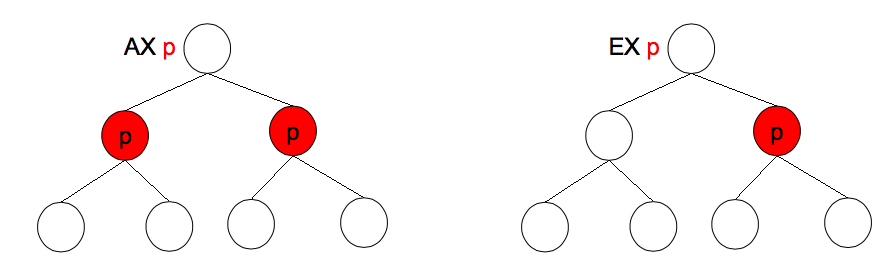
\includegraphics[width=130mm]{15/images/temporal}
\end{figure}
